\documentclass[prb,11pt]{revtex4-1}

% preamble:

\usepackage{amsmath}    % need for subequations
\usepackage{graphicx}   % need for figures
\usepackage{verbatim}   % useful for program listings
\usepackage{color}      % use if color is used in text
\usepackage{subfigure}  % use for side-by-side figures
\usepackage{hyperref}   % use for hypertext links, including those to external documents and URLs
\raggedbottom           % don't add extra vertical space
\begin{comment}
\pagestyle{empty}       % use if page numbers not wanted
\end{comment}

\begin{document}

\title{Effective viscosity of polymer networks in the presence of cross-link slip}
\author{William McFadden}
\affiliation{University of Chicago, Biophysical Sciences Program, Chicago, IL 60615}

\date{1 January 2014}

\begin{abstract}
We are trying to describe the problem of what happens when cross-links relax stress in semi-flexible filament networks.  We have addressed the problem using a simplified model in which cross-links are allowed to slip past one another in a friction-like manner.  This model gives a prediction for the long timescale effective viscosity of the medium.  We have verified our solution using computational models of filaments in the limit where persistence length is much longer than filament length.  In this model, we find that network architectures and slip rates give rise to different modes of connectivity.
\end{abstract}

\maketitle

\section{Introduction}

In previous work, crosslinks have been taken to be either perfectly rigid attachment points (HLM) or extended springlike structures (Taeyoon).  In addition, any mechanism of detachment is either absent (HLM) or governed by full detachment and full reattachment events (Taeyoon, Broederz).  In our model, we aim to create a more simple and general picture of crosslink stress relaxation based on an effective molecular friction between filament attachment points.

Previous researchers have introduced the concept of molecular friction to describe crosslink slip.  We want to look at what such a model would produce in a larger network.

Chemists have made synthetic systems that exhibit so called slide-ring cross-linking, but thus far this exact mechanism has not been seen in biological systems.  However, (some garbage experiments from biophysical journal that I know must exist because people put bullshit in biophysical journal all the time) have shown that multivalent crosslinks can effectively slide under a load.


\section{The Model}

In the worm-like chain model, semi-flexible polymers are modeled as continuous curves, governed by a potential 
\begin{equation}
{\cal H} =\frac{1}{2}\kappa \int ds(\nabla^2\mathbf{u})^2 + \frac{1}{2}\mu \int ds \left ( \frac{dl(s) }{ds} \right )^2
\end{equation}

We generate 2D networks of these semi flexible filaments by laying them down with random position and orientation.  

Although real cytoskeletal networks may exhibit non-negligible anisotropy, we choose to focus our attention on isotropic networks for simplicity.  We define the density using the distance between crosslinks along a filament, $l_c$. A simple geometrical argument can be used to prove that the number of filaments needed to fill a domain of size 2D x D is $4D^2/Ll_c$. 

In the absence of crosslink slip, we expect the network to comprise a connected solid with a well defined elastic modulus given by HLM.  These networks are only well-connected when the ratio of filament length to intercrosslink spacing, $L/l_c$ is greater than ~5.6.  Below this percolation threshold, there are only locally connected domains.  Additionally, as the filament density is increased beyond this point, there is another transition between non-affine bending and affine stretching of filaments, which changes the dominating term of the elastic modulus.

In departure from the previous models, we wish to incorporate relaxation of the networks stored stress by letting the attachment points slip.  We do this by introducing a frictional coupling between filaments.
\begin{equation}
\mathbf{F_{friction}} = \delta \zeta \cdot \int ds \: (\mathbf{v(s)}-\mathbf{v_0(s)}) \: p(s)
\end{equation}

In this case the motion for the entire network is governed by a dynamical equation of the form

\begin{equation}
\zeta \int ds \: (\mathbf{v_i(s)} + \delta \sum _j(\mathbf{v_i(s)}-\mathbf{v_j(s)}) \: p_{ij}(s))= \nabla {\cal H}_i
\end{equation}

Although the general mechanical response of this system may be very complex, we wish to focus our attention on the linear order steady-state creep response of the system to an applied stress.  To do this we introduce a spatially varying stress along the midline of our domain.

\begin{equation}
F_{total}= \nabla {\cal H}_i + \sigma(x)-\zeta \int ds \: (\mathbf{v_i(s)} + \delta \sum _j(\mathbf{v_i(s)}-\mathbf{v_j(s)}) \: p_{ij}(s)) 
\end{equation}

Finally, we add a 0 velocity constraint at the far edges of our domain of interest.  We assume that our network is in the low Reynold's number limit, where inertial effects are so small that we can equate our total force to 0.  The above equation is then discretized and integrated in time to determine the material response.

\section{Analytical Results}
We would like to calculate an estimate of the effective viscosity for a network described by our model.  We carry this out by assuming we can apply a constant stress along a transect of the network.  With moderate stresses, we assume the network reaches a steady state affine creep. In this situation, we would find that the stress in the network exactly balances the sum of the frictional forces from crosslink slip.  So for any transect of length D, we have a force balance equation.

\begin{equation}
\mathbf{\sigma} = \frac{1}{D}\sum_{filaments}\: \sum_{crosslinks}\delta \zeta \cdot (\mathbf{v_i}-\mathbf{v_0})
\end{equation}

where $\mathbf{v_i(s)}-\mathbf{v_j(s)}$ is the difference between the velocity of a filament at it's crosslink point and the velocity of the filament to which it is a attached. We can convert the sum over crosslinks to an integral over the length using the average density of crosslinks, $1/l_c$ and invoking the assumption of (linear order) affine strain rate, $\mathbf{v_i}-\mathbf{v_0}=\dot \gamma x$. This results in

\begin{equation}
\mathbf{\sigma} =  \frac{1}{D}\sum_{filaments}\:  \delta \zeta \cdot \int_0^L ds \: (\mathbf{v(s)}-\mathbf{v_0(s)}) \:\frac{1}{l_c} = \sum_{filaments}\:  \frac{\delta \zeta \dot \gamma L}{l_c} \cos \theta \cdot (x_l + \frac{L}{2} \cos \theta)
\end{equation}

Here we have introduced the variables $x_l$, and $\theta$ to describe the leftmost endpoint and the angular orientation of a given filament respectively.  Next, to perform the sum over all filaments we wish to convert this to an integral over all orientations and endpoints that intersect our line of stress. The max distance for the leftmost endpoint is the length of a filament, L, and the maximum angle as a function of endpoint is $\arccos(x_l/L)$.  The linear density of endpoints is the constant $D/l_cL$ so our integrals can be rewritten as this density over $x_l$ and $\theta$ between our maximum and minimum allowed bounds.

\begin{equation}
\mathbf{\sigma} =  \frac{1}{D} \int_0^L dx_l \int_{-\arccos (\frac{x_l}{L})}^{\arccos (\frac{x_l}{L})}d\theta \frac{\delta \zeta \dot \gamma L}{l_c} \cdot \frac{D}{Ll_c}\cdot (x_l \cos \theta + \frac{L}{2} cos^2\theta)
\end{equation}

Carrying our the integrals leaves us with a relation between stress and strain rate.

\begin{equation}
\mathbf{\sigma} = \frac{4L^2\delta \zeta}{3l_c^2} \dot \gamma \end{equation}

We recognize that the term next to the strain rate is the effective viscosity $\eta_{eff}$ at steady state creep.  With the constitutive relation for the rate of deformation, we can next write down an equation for the rate of network thinning.  

\begin{equation}
\frac{\partial l_c}{dt}=l_c\dot \gamma =\frac{l_c \sigma}{\eta}=l_c^3\frac{ \sigma}{L^2 \delta \zeta}
\end{equation}

We can see that the rate of network thinning accelerates as we would expect.  When the network reaches some minimum connectivity we assume that it stops behaving as a continuum material.  

\begin{equation}
\tau_{break} = \frac{\eta_{eff}}{2\sigma}\cdot\left ( 1 -\frac{l_c^2}{l_{break}^2} \right )
\end{equation}

This provides us with an estimate of the timescale of catastrophic breakdown for a network with a given initial architecture and molecular friction.

Finally, we wish to extend this analysis to have some idea of the frequency dependence of the complex elastic modulus.  I sure hope there is some way to do this.


\section{Computational Simulations}

Next, we wanted to test our analytical conclusions on a computational model.  The technical details of the model can be found in the Appendix, but we summarize the main modeling points here.

For computational simplicity in these models, we assume that the bending rigidity, $\kappa$, is infinite, allowing us to model filaments as non-bending springs of rest length, $L$, and spring modulus $\mu$.  In the appendix, we show that our result is not significantly different from the result for semi-flexible polymers.

We discretize the filaments such that the equations of motion becomes a coupled system of equations for the velocities of filament endpoints, $\mathbf{x}$.  The frictional force between overlapping filaments results in a coupling of the velocities of endpoints.  

\begin{equation}
\mathbf{A \cdot \dot x} = \mathbf{f(x)}
\end{equation}

where $\mathbf{A }$ represents a coupling matrix between endpoints of filaments that overlap, and $\mathbf{f(x)}$ is the spring force between two endpoints.  We can then numerically integrate this system of equations to find the time evolution of the positions of all filament endpoints.

We generate a network by laying down filaments with random position and orientation within a domain of size $2D$ by $D$ with periodic boundaries.  The external stress (shear or extensional/compressional) is applied to all filament endpoints falling within a fixed x-distance from the center of the domain.  Finally, filament endpoints falling within a fixed x-distance from the edges of the domain are constrained to be nonmoving.

\begin{figure}[h!]
\centering
\includegraphics[width=\textwidth]{simuls}
\caption{\label{fig:sim}Two Simulation setups with $L=16 \mu m, D = 64 \mu m$. a) low density $l_c=2 \mu m$, b) high density $l_c=0.25 \mu m$ }
\end{figure}


All changes in the force felt by an endpoint are made smooth to allow integration of the differential equation (i.e. moving between stress domains, constraint domains, and overlap coupling occurs smoothly to prevent discontinuities).  Parameter conditions that cause instabilities are excluded, and the endpoint trajectories are integrated out to at least 1000 seconds. 


\section{Simulation Results}

And here, I show the simulation results, which fall into three categories, 1) the steady state effective viscosity matches the theoretical prediction in a range of parameter space, 2) the network tearing time drops as the effective viscosity drops to 0, 3) the frequency falloff can be explained by heterogeneity in length, 

\begin{figure}[h!]
\centering
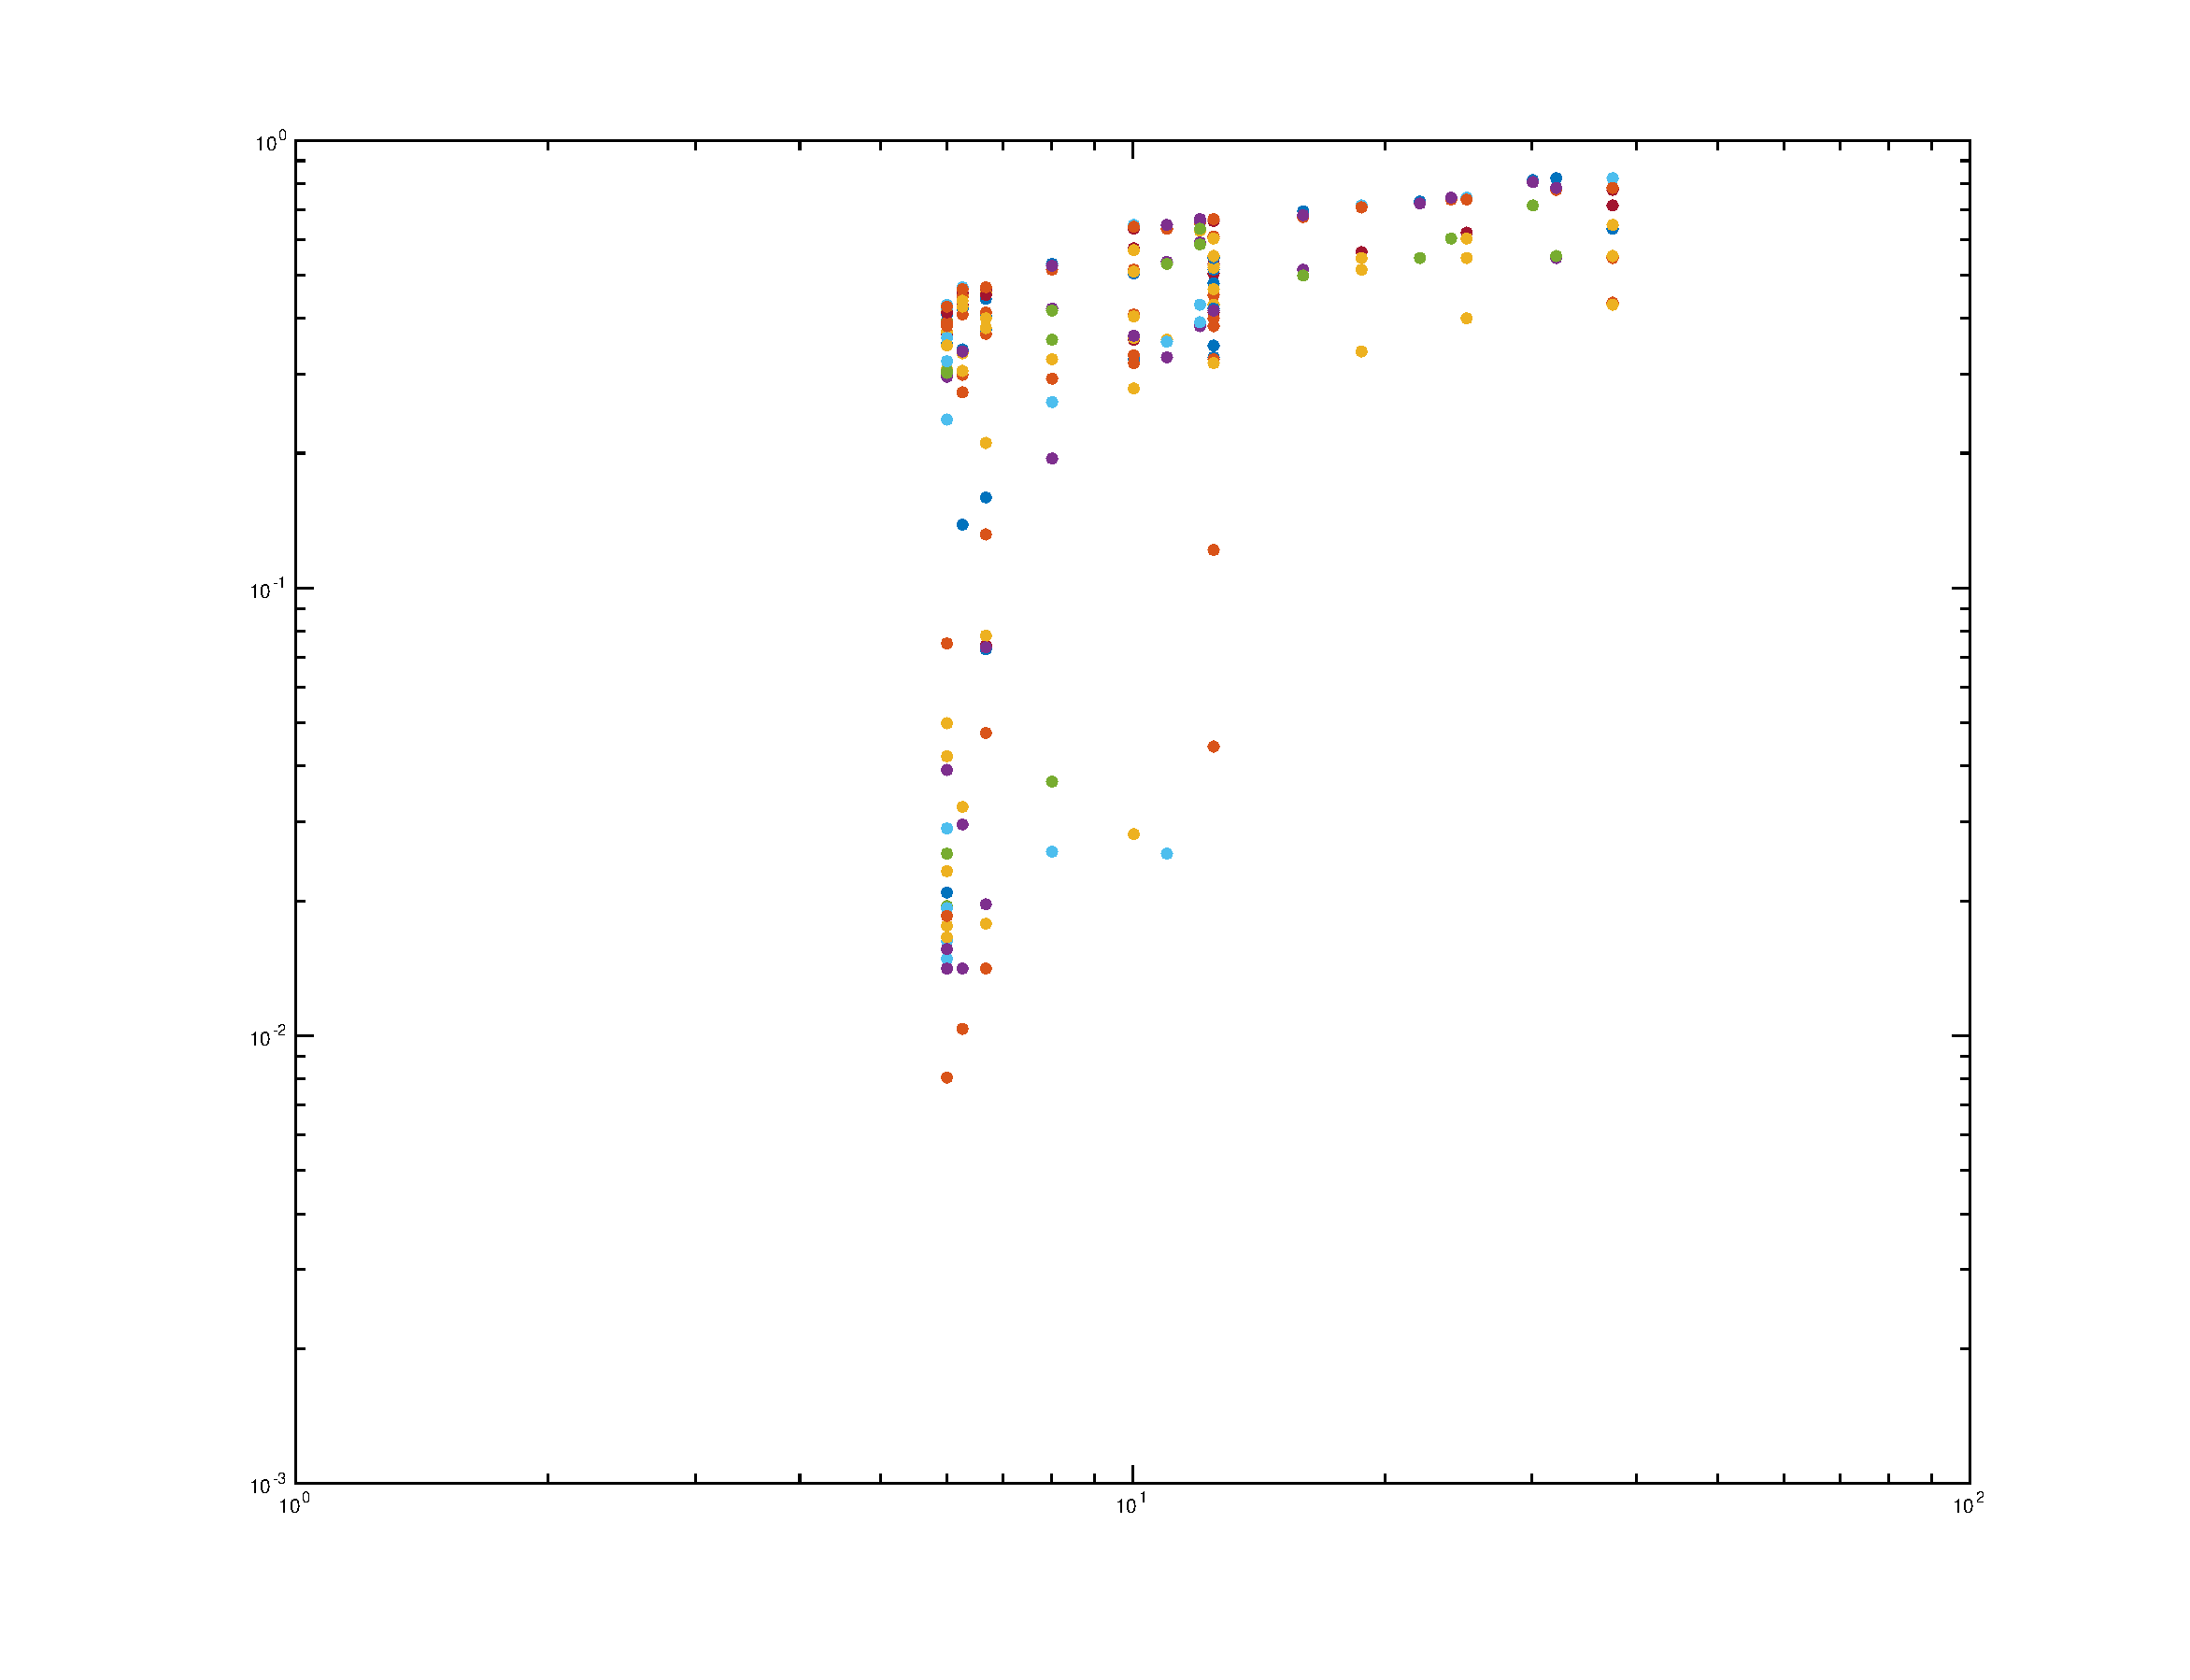
\includegraphics[width=\textwidth]{eff_vic}
\caption{\label{fig:effvic}Effective viscosity as a function of $L/l_c$.}
\end{figure}

\begin{figure}[h!]
\centering
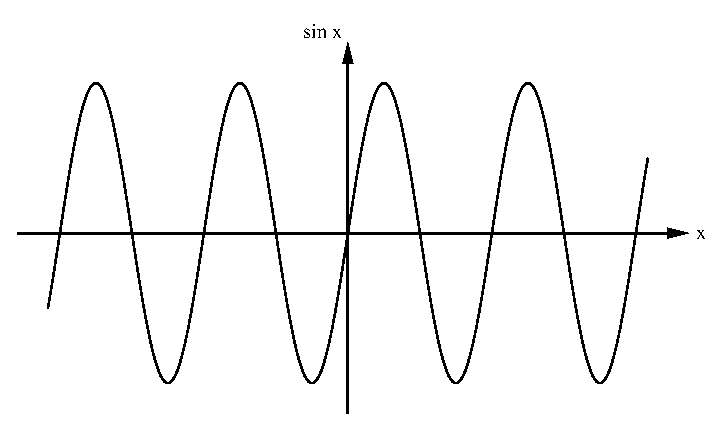
\includegraphics[scale=0.6]{sine}
\caption{\label{fig:tear}Tearing rate as a function of $L/l_c$.}
\end{figure}

\begin{figure}[h!]
\centering
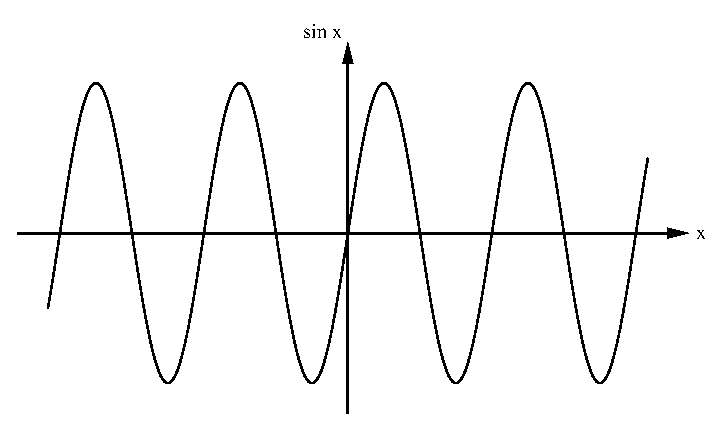
\includegraphics[scale=0.6]{sine}
\caption{\label{fig:freq}Frequency dependence of elastic moduli.}
\end{figure}




\section{Discussion}

{\color{blue}{Finally I wax philosophical}},
{\color{green}{but}} {\color{cyan}{who is going to pay for the ink?}}

\begin{figure}[h!]
\centering
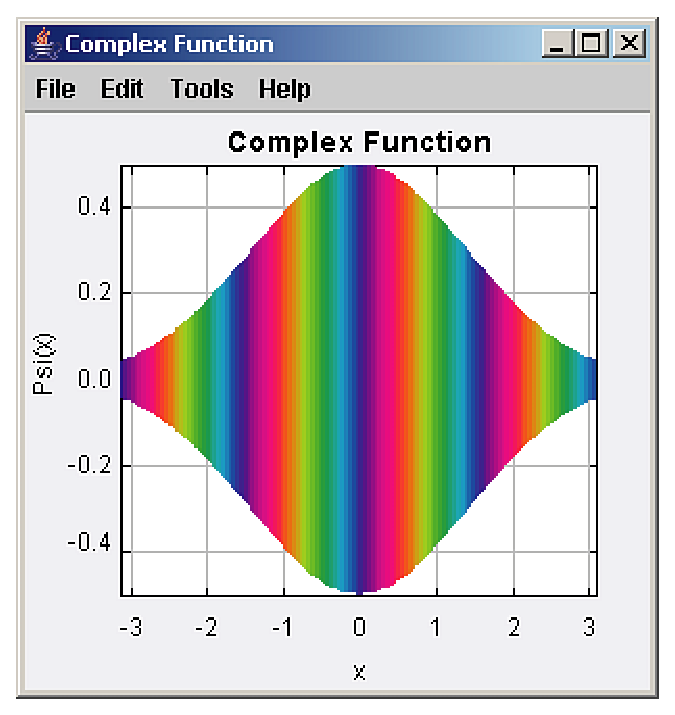
\includegraphics[scale=0.6]{phase}
\caption{\label{fig:sim}Phase diagram of network connectivity.}
\end{figure}

\section{Appendix A: Deriving molecular friction coefficients}
Thus far, the idea of a molecular friction coefficient was taken as a phenomenological, measured parameter for a given experimental setup.  While this is a sufficient pragmatic justification, it's useful to try to motivate the quantitative value of this friction coefficient by connecting it to the underlying cross-link properties of binding affinity, concentration, and extensibility.

To do this we'll imagine the simplified case of two cross linkers sliding past each other in one dimension.  In this case, imagine that we have an equilibrium number of bound crosslinkers, $n_B$, each of which can be displaced from its equilibrium length by some distance $x$.  Each cross linker unbinds with rate $k_{off}$ and rebinds at it's relaxed position ($x=0$) with rate $k_{on}$.  At the same time, all the cross linkers are being pulled from their relaxed position at a rate, $v$, which is simply the rate at which the filaments are sliding past each other.  

We can right down an equation for the change in the density of crosslinks as they are advected, bind, and unbind.

\begin{equation}
\frac{\partial \rho}{\partial t} = -k_{off}\rho(x) - v\frac{\partial \rho}{\partial x} + k_{on}\delta(x)
\end{equation}

Recognizing that $\int \rho(x)=n_B$ implies $k_{on}=k_{off}n_B$, we can find the steady state solution

\begin{equation}
\rho(x) = \frac{n_b k_{off}}{v}\cdot exp\left ( -\frac{k_{off}}{v}x \right )
\end{equation}

If each crosslink has a spring constant $\mu_c$, then we can equate the force on all crosslinks to the applied force that is sliding the filaments past each other.

\begin{equation}
\int_{0}^{\infty}\rho(x)\mu_cx dx = v \frac{\mu_c n_B}{k_{off}}= F_{app}
\end{equation}

Therefore, the term next to v, (i.e. $\tfrac{\mu_c n_B}{k_{off}}$) would be equal to our molecular friction coefficient, $\delta\zeta$.  Using the following table of estimates cobbled from a variety of data sources, we can chart the accuracy of this simple predictive model.

\section{Appendix B: Simulation details}
And I think I'll probably include all the gory details of how my simulations work since I'll be wanting to have direct references to the code. 
\begin{verbatim}
double y0 = 10; // example of declaration and assignment statement
double v0 = 0;  // initial velocity
double t = 0;   // time
double dt = 0.01; // time step
double y = y0; // solved all problems
\end{verbatim}




\begin{thebibliography}{5}

\bibitem{latex}Helmut Kopka and Patrick W. Daly, \textsl{A Guide to
\LaTeX: Document Preparation for Beginners and Advanced Users} (Addison-Wesley, 2004), 4th ed.

\bibitem{website}Some useful links are
given at \url{<sip.clarku.edu/tutorials/TeX/>}.

\end{thebibliography}

\end{document}